\documentclass[resume]{subfiles}



\begin{document}
\section{Espaces d'états}
\begin{figure}[H]
\centering
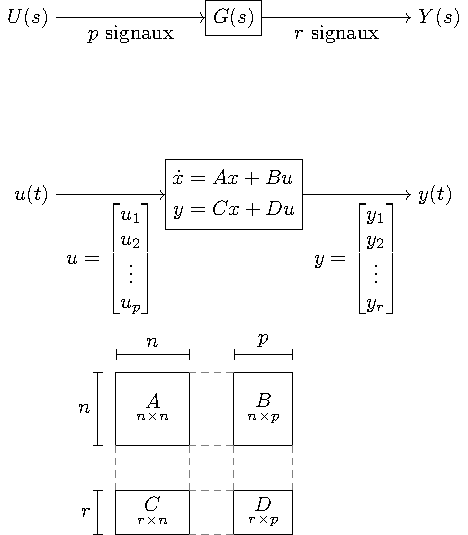
\includegraphics[scale=1,page=1]{drwg_0.pdf}
\end{figure}
\subsection{Choix des variables d'état}
\begin{itemize}
\item Condensateur : tension
\item Bobine : courant
\end{itemize}


\subsection{$A,B,C,D \longrightarrow G$}
$$G(s)=C(sI-A)^{-1}B+D$$
$$G(z)=C_n(zI-A_n)^{-1}B_n+D_n$$
\subsubsection{Gain haute fréquence}
$$\lim_{s\to\infty}G(s)=D$$
\subsubsection{Gain basse fréquence}
$$G(0)=-CA^{-1}B+D$$
\subsection{$G\longrightarrow A,B,C,D$}
On utilise la forme commandable
$$G(s)=\frac{b_2s^2+b_1s+b_0}{s^3+a_2s^2+a_1s+a_0}$$
$$\boxed{\begin{split}
A&=\begin{bmatrix}0 & 1 & 0\\0 & 0 &1\\-a_0 & -a_1 & -a_2\end{bmatrix} &
B&= \begin{bmatrix}
0\\0\\1
\end{bmatrix}\\
C&=\begin{bmatrix}b_0 & b_1 & b_2\end{bmatrix} & D&=0\end{split}}$$
\subsection{$G(s) / G(z) \longleftrightarrow A,B,C,D$}
\begin{figure}[H]
\centering
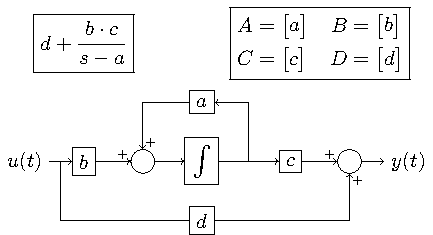
\includegraphics[scale=1,page=1]{drwg_1.pdf}\\
\includegraphics[scale=1,page=2]{drwg_1.pdf}
\end{figure}

\subsection{Mise en cascade}
\begin{figure}[H]
\centering
\includegraphics[scale=1,page=2]{drwg_0.pdf}
\end{figure}
$$S_{tot}=S_2(s)\cdot S_1(s)\qquad\text{ordre important}$$
$$A_{tot}=\begin{bmatrix}
A_1 & 0\\
B_2C_1 & A_2
\end{bmatrix}\qquad B_{tot}=\begin{bmatrix}
B_1\\B_2D_1
\end{bmatrix}$$
$$C_{tot}=\begin{bmatrix}
D_2C_1 & C_2
\end{bmatrix}\qquad D_{tot}=D_2D_1$$
\subsection{Mise en parallèle}
\begin{figure}[H]
\centering
\includegraphics[scale=1,page=3]{drwg_0.pdf}
\end{figure}
$$S_{tot}(s)=S_1(s)+S_2(s)$$
$$A_{tot}=\begin{bmatrix}
A_1 & 0\\0 & A_2
\end{bmatrix}\qquad B_{tot}=\begin{bmatrix}
B_1\\B_2
\end{bmatrix}$$
$$C_{tot}=\begin{bmatrix}
C_1 & C_2
\end{bmatrix}\qquad D_{tot}=D_1+D_2$$
\subsubsection{Mise en contre-réaction 1}
\begin{figure}[H]
\centering
\includegraphics[scale=1,page=4]{drwg_0.pdf}
\end{figure}
$$A_{tot}=\begin{bmatrix} A_1 - B_1D_2(I-D_1D_2)^{-1}C_1 & -B_1(C_2-D_2D_1C_2)\\B_2(I-D_1D_2)^{-1}C_1 & A_2-B_2(I-D_1D_2)^{-1}D_1C_2\end{bmatrix}\qquad B_{tot}=\begin{bmatrix}B_1-B_1D_2ND_1\\B_2ND_1\end{bmatrix}$$

$$C_{tot}=\begin{bmatrix}(I-D_1D_2)^{-1}C_1 & -(I-D_1D_2)^{-1}D_1C_2\end{bmatrix}\qquad D_{tot}=(I-D_1D_2)^{-1}D_1$$ 

\subsubsection{Mise en contre-réaction 2}
\begin{figure}[H]
\centering
\includegraphics[scale=1,page=5]{drwg_0.pdf}
\end{figure}
$$S_{tot}(s)=\left(I+S_1(s)S_2(s)\right)^{-1}S_1(s)$$
$$A_{tot}=\begin{bmatrix}A_1 & 0\\B_2C_1 & A_2\end{bmatrix}\qquad B_{tot}=\begin{bmatrix}B_1\\B_2D_1\end{bmatrix}$$
$$C_{tot}=\begin{bmatrix}
D_2 C_1 & C_2
\end{bmatrix}\qquad D_{tot}=D_1D_2$$
\subsection{Commandabilité}
$$\boxed{P_c=\begin{bmatrix}B & AB & \cdots & A^{n-1}B\end{bmatrix}}$$
Pour des systèmes monoentrée :
$$\det(P_c)\neq 0\longrightarrow \text{Commandable}$$
Pour des systèmes multi-entrées (généralisation) :
$$\text{rang}(P_c)==n\longrightarrow \text{Commandable}$$
Faire une permutation avec $T$ ne change pas la commandabilité du système. La nouvelle matrice $\tilde{P}_c$ est donnée par $T^{-1}P_c$
\subsection{Observabilité}
$$\boxed{P_0=\begin{bmatrix}C\\CA\\CA^2\\\vdots\\CA^{n-1}\end{bmatrix}}$$
$$\boxed{\text{rang}(P_0)=n\longrightarrow\text{Observable}}$$
En monosortie on peut utiliser $\det(P_0)\neq 0\longrightarrow \text{Observable}$


\subsection{Action intégrale sur la commande}
\begin{figure}[H]
\centering
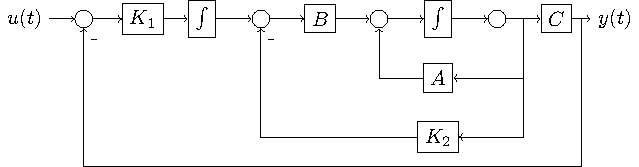
\includegraphics[width=\columnwidth]{drwg_2.pdf}
\end{figure}
$$\hat{A}=\begin{bmatrix}0 & C\\0 & A\end{bmatrix}\qquad B=\begin{bmatrix}0\\b\end{bmatrix}$$
\subsection{Placement de pôles}
Il faut que le polynôme caractéristique de la boucle fermée (par exemple $sI-A_{bf}=sI-(A-BK)$) corresponde aux pôles que l'ont souhaite
$$\det(sI-A_{bf})=(s-p_1)(s-p_2)\cdots(s-p_n)$$
\end{document}